\documentclass[11pt,a4paper]{article}
\newcommand{\ReportFooter}{설원경 멀티플레이 서버}
\usepackage[margin=20mm, top=19mm, bottom=20mm]{geometry}
\usepackage{fontspec}
\setmainfont{texgyrepagella}[
  Extension=.otf, UprightFont=*-regular, ItalicFont=*-italic,
  BoldFont=*-bold, BoldItalicFont=*-bolditalic]
\setsansfont{texgyreheros}[
  Extension=.otf, UprightFont=*-regular, ItalicFont=*-italic,
  BoldFont=*-bold, BoldItalicFont=*-bolditalic]
\usepackage{amsmath}
\usepackage{graphicx}
\graphicspath{{../images/}}
\usepackage{booktabs, tabularx}
\usepackage{caption}
\usepackage{enumitem}
\usepackage{placeins}
\usepackage{titlesec}
\usepackage{fancyhdr}
\usepackage{cite}
\usepackage{xcolor}
\usepackage{xurl}
\usepackage[unicode]{hyperref}

\definecolor{accent}{HTML}{204E77}
\definecolor{muted}{HTML}{455464}
\definecolor{rulegray}{HTML}{CAD3DC}
\hypersetup{colorlinks=true, linkcolor=accent, citecolor=accent, urlcolor=accent}
\urlstyle{same}

\setlength{\parindent}{0pt}
\setlength{\parskip}{5.5pt plus 1pt}
\linespread{1.05}
\raggedbottom
\clubpenalty=10000
\widowpenalty=10000
\setlist{topsep=2pt, itemsep=2pt, parsep=0pt, leftmargin=1.65em}
\setlength{\textfloatsep}{14pt plus 2pt minus 3pt}
\setlength{\intextsep}{12pt plus 2pt minus 2pt}
\setlength{\tabcolsep}{5pt}
\renewcommand{\arraystretch}{1.25}
\newcolumntype{L}{>{\raggedright\arraybackslash}X}
\newcolumntype{P}[1]{>{\raggedright\arraybackslash}p{#1}}
\captionsetup{font=small, labelfont=bf, labelsep=period, justification=raggedright,
  singlelinecheck=false, skip=7pt}
\AddToHook{env/thebibliography/begin}{\small\raggedright}

\titleformat{\section}{\Large\sffamily\bfseries\color{accent}}{\thesection}{0.65em}{}
\titleformat{\subsection}{\large\sffamily\bfseries}{\thesubsection}{0.65em}{}
\titlespacing*{\section}{0pt}{15pt plus 2pt minus 2pt}{5pt}
\titlespacing*{\subsection}{0pt}{11pt plus 2pt minus 2pt}{3pt}

\pagestyle{fancy}
\fancyhf{}
\renewcommand{\headrulewidth}{0pt}
\renewcommand{\footrulewidth}{0.3pt}
\fancyfoot[L]{\sffamily\small\color{muted}\ReportFooter}
\fancyfoot[R]{\sffamily\small\color{muted}\thepage}

\newcommand{\ReportTitle}[3]{%
  {\sffamily\bfseries\small\color{accent}#1\par}
  \vspace{5pt}
  {\sffamily\bfseries\fontsize{22}{27}\selectfont\raggedright #2\par}
  \vspace{4pt}
  {\sffamily\small\color{muted}#3\par}
  \vspace{2pt}
  {\color{rulegray}\hrule}
}

\newcommand{\code}[1]{\texttt{#1}}
\newcommand{\change}[2]{#1 \(\to\) #2}

\newcommand{\ReportFigure}[3]{%
  \par\medskip
  \noindent\begin{minipage}{\linewidth}
    \captionsetup{type=figure}
    \includegraphics[width=\linewidth]{#1}\par
    \caption{#2}
    \label{#3}
  \end{minipage}\par
}

\newcommand{\DeltaRows}{%
   50 & \change{62.5}{27.6} & \change{3.05}{1.35} \\
  100 & \change{65.3}{28.9} & \change{6.38}{2.82} \\
  200 & \change{70.8}{28.4} & \change{13.83}{5.54} \\
  400 & \change{54.5}{23.4} & \change{21.30}{9.14} \\
}

\newcommand{\UbuntuRows}{%
    400 &  47\% & 14.5 & 40 / 74 \\
    800 & 100\% & 13.6 & 49 / 91 \\
  1,000 & 133\% & 11.8 & 55 / 103 \\
  1,200 & 125\% &  7.8 & 161 / 237 \\
}

\newcommand{\StageRows}{%
  100 & 14.5 / 71  & 15.0 / 71  & \change{19\%}{11\%} \\
  200 & 14.0 / 77  & 15.0 / 74  & \change{37\%}{19\%} \\
  400 & 10.8 / 296 & 15.0 / 78  & \change{63\%}{33\%} \\
  800 &  8.0 / 725 & 15.0 / 325 & \change{71\%}{48\%} \\
}

\newcommand{\ProductionRows}{%
    200 & 15.0 & 39 / 75          & 71\%          & 30\%         & 26\% \\
    400 & 15.0 & 49 / 85          & 113\%         & 58\%         & 47\% \\
    600 & 15.0 & 52--53 / 95--98  & 158--161\%    & 87--90\%     & 63--65\% \\
    700 & 15.0 & 57 / 114         & 180\%         & 101\%        & 73\% \\
    800 & 15.0 & 75--101 / 163--275 & 189--197\%  & 90--108\%    & 87--94\% \\
  1,000 & 12.7 & 237 / 3,467      & 197\%         & 100\%        & 91\% \\
  1,200 & 14.3 & 445 / 1,309      & 200\%         & 92\%         & 91\% \\
}

\usepackage{xetexko}
\setmainhangulfont{UnBatang.ttf}[
  BoldFont=UnBatangBold.ttf, ItalicFont=UnBatang.ttf,
  BoldItalicFont=UnBatangBold.ttf]
\setsanshangulfont{UnDotum.ttf}[BoldFont=UnDotumBold.ttf]
\renewcommand{\figurename}{그림}
\renewcommand{\tablename}{표}
\renewcommand{\refname}{참고문헌}
\hypersetup{
  pdftitle={설원경 멀티플레이 서버의 성능 최적화와 부하 시험},
  pdflang={ko}
}

\begin{document}
\ReportTitle{학술 재구성본}
  {설원경 멀티플레이 서버의\\성능 최적화와 부하 시험}
  {운영 서버 부하 시험 \enspace\textbar\enspace 2026년 11월 14일}

\pdfbookmark[1]{초록}{abstract}
\section*{초록}
본 보고서는 한국어 메타버스 스키장 서비스 설원경(\href{https://ski.stelide.com}{ski.stelide.com})의 멀티플레이 서버를 대상으로 부하 시험을 수행하고, 발견된 병목을 순차적으로 제거한 과정과 결과를 다룬다. 2코어(Oracle Ampere) 운영 서버에서 동시 접속자 수를 단계적으로 증가시키며 위치 전달 지연, 갱신 빈도, 송수신량, 프로세스별 CPU 사용량을 측정했다. 파이썬 구현은 약 450명까지 원활할 것으로 추정되었다. 네 가지 최적화, 즉 (1) 위치 전체 대신 변경된 필드만 전송하는 델타 인코딩, (2) 데이터베이스 연결 누수로 인한 파일 핸들 고갈 수정, (3) 접속 한도 상향(400명에서 2,000명), (4) 실시간 중계의 Go 재구현을 거쳐 동시 접속 700명에서 위치 전달 지연 p99 114\,ms, 초당 15회 갱신을 달성했다. 800명에서 CPU가 포화에 가까워졌고 1,000명부터 지연이 초 단위로 증가했다. TLS를 제외한 시험 경로에서 원활 기준을 충족한 최대 부하는 700명이었다. 본 사례는 관심 영역 관리 및 증분 상태 전송 기법이 소규모 상용 서비스의 실측 환경에서도 유효함을 보여준다.

{\small\textbf{주요어} \quad 메타버스 서버, 성능 최적화, 부하 시험, 관심 영역 관리, 증분 상태 전송}

\section{서론}
설원경은 실시간으로 여러 사용자의 아바타 위치를 주고받는 멀티플레이 기능을 포함하는 메타버스 스키장 서비스다. 실시간 위치 중계는 접속자 수가 늘어날수록 CPU와 대역폭을 소모하며, 서비스 규모가 커질수록 가장 먼저 포화되는 구성 요소다. 본 보고서의 목적은 (1) 운영 서버의 동시 접속 한계를 측정하고, (2) 병목을 식별하여 제거하며, (3) 남은 한계와 다음 대응 전략을 정량적으로 남기는 것이다.

본 연구의 기여는 다음 네 가지다. 첫째, 게임 엔진과 동일한 움직임을 재현하는 부하 시험 하네스를 설계하여 측정 왜곡의 원인(하네스와 서버 틱의 동기화, 동일 머신 측정)을 식별하고 보정했다. 둘째, 변경 필드만 전송하는 델타 인코딩 도입으로 1인당 수신량을 56--60\% 감소시켰다. 셋째, 파일 핸들 누수와 접속 한도라는 두 가지 병목을 진단하고 수정했다. 넷째, 파이썬 GIL에 의한 확장성 한계를 실측으로 확인하고 실시간 중계만 Go로 재구현했다. STAGE에서 Go 중계의 1인당 CPU 사용량은 파이썬의 약 \(1/2.2\)였으며, 운영 서버에서 실측한 원활 수용 인원은 파이썬 추정치의 약 1.5배였다.

\section{관련 연구}
다중 사용자 온라인 게임의 서버 확장성은 오래된 연구 주제다. 클라이언트-서버(CS) 구조는 중앙 서버의 대역폭 요구량이 플레이어 수에 따라 비례 이상으로 증가하기 때문에 확장성이 제한된다. 피어 간 상태 일관성 검사 비용과의 균형을 분석한 연구에서 CS 구조의 서버 대역폭 병목이 지적되었다~\cite{pellegrino_2003_12}. 이를 완화하는 대안으로 서버-피어 혼합 구조가 제안되었다~\cite{kim_2013}.

이러한 병목의 표준 해법은 관심 영역 관리(interest management)다. 대규모 분산 시뮬레이션에서 모든 상태 변화를 모든 참여자에게 방송하면 수신 메시지가 급증하므로, 각 참여자에게 관련 있는 부분만 필터링하여 전달하는 기법이 체계화되었고~\cite{morse_2000_1}, 이후 설계 분류와 트레이드오프를 정리한 종설이 제시되었다~\cite{liu_2014_2}. 실제 게임에서 측정한 연구는 장애물을 고려한 관심 영역 알고리즘이 갱신 메시지 수를 최대 6배까지 줄이며, 계산 비용이 작은 타일 기반 알고리즘이 이상적인 가시성 기반 기법을 낮은 비용으로 근사함을 보였다~\cite{boulanger_2006_10}. 클라우드 환경에서 발행-구독 기반 관심 집합으로 대역폭을 줄여 수백 명 규모까지 확장한 사례도 있다~\cite{najaran_2010_5}. 대역폭 할당량을 유지하며 상태 갱신 메시지를 적응적으로 필터링하는 미들웨어도 제안되었다~\cite{gascon_samson_2015_6}.

본 보고서의 첫 번째 최적화인 델타 인코딩(변경 필드만 전송)은 증분 상태 전송의 단순한 형태다. 예측, 학습, 엔트로피 부호화로 증분 상태 표현을 학습하여 수백 개 개체를 초당 수 킬로바이트 미만으로 동기화한 연구~\cite{orsten_2011_4}와, 시간 상관을 이용한 델타 부호화로 동적 웹 콘텐츠의 대역폭 요구량을 줄인 연구~\cite{psounis_2002_11}가 같은 원리를 활용한다. 기존 문헌에서는 대규모 MMOG와 분산 시뮬레이션을 시뮬레이션이나 테스트베드에서 주로 평가해 왔다. 본 보고서는 소규모 상용 서비스의 운영 서버에서 nginx와 커널 네트워크 처리를 포함해 실측했다. 구현 언어 수준의 병목(GIL)과 리버스 프록시 비용도 정량화했다.

\section{시스템 구조}
실시간 위치 중계는 Go 프로그램이 담당하며, 방(room) 단위로 위치 갱신을 모아 초당 15회(15\,Hz) 방 전원에게 동일 프레임으로 송신한다. 페이지, 로그인, 랭킹, 데이터베이스 처리는 파이썬 서버가 유지한다. 슬로프 채널 방 하나의 수용 인원은 40명(서버 상한 48명)이고 파티는 별도 방을 사용한다. 그림~\ref{fig:architecture}는 실제 플레이어의 접속 경로를 보여준다.

프로토콜은 세 종류 메시지로 구성된다. 입장 시 1회 전체 상태(\code{u})를 보내고, 이후에는 변경된 필드만(\code{v}) 보내며, 퇴장은 \code{x}로 알린다. 서버는 1/15초마다 방 내 위치가 변한 참여자들을 하나의 프레임으로 묶는다. 앞뒤가 맞지 않는 비정상적으로 급격한 위치 변화는 중계하지 않으며, 충돌 판정도 서버가 속도와 거리로 수행하는 서버 권위적(server-authoritative) 구조다. 서버 전체 동시 접속 상한은 2,000명이고 IP당 접속 수, 접속당 메시지 속도에도 제한이 있다. 이전 파이썬 중계 구현을 그대로 보존해 두어, 문제 발생 시 nginx 설정 한 줄로 롤백할 수 있다.

\begin{figure}[!htbp]
  \centering
  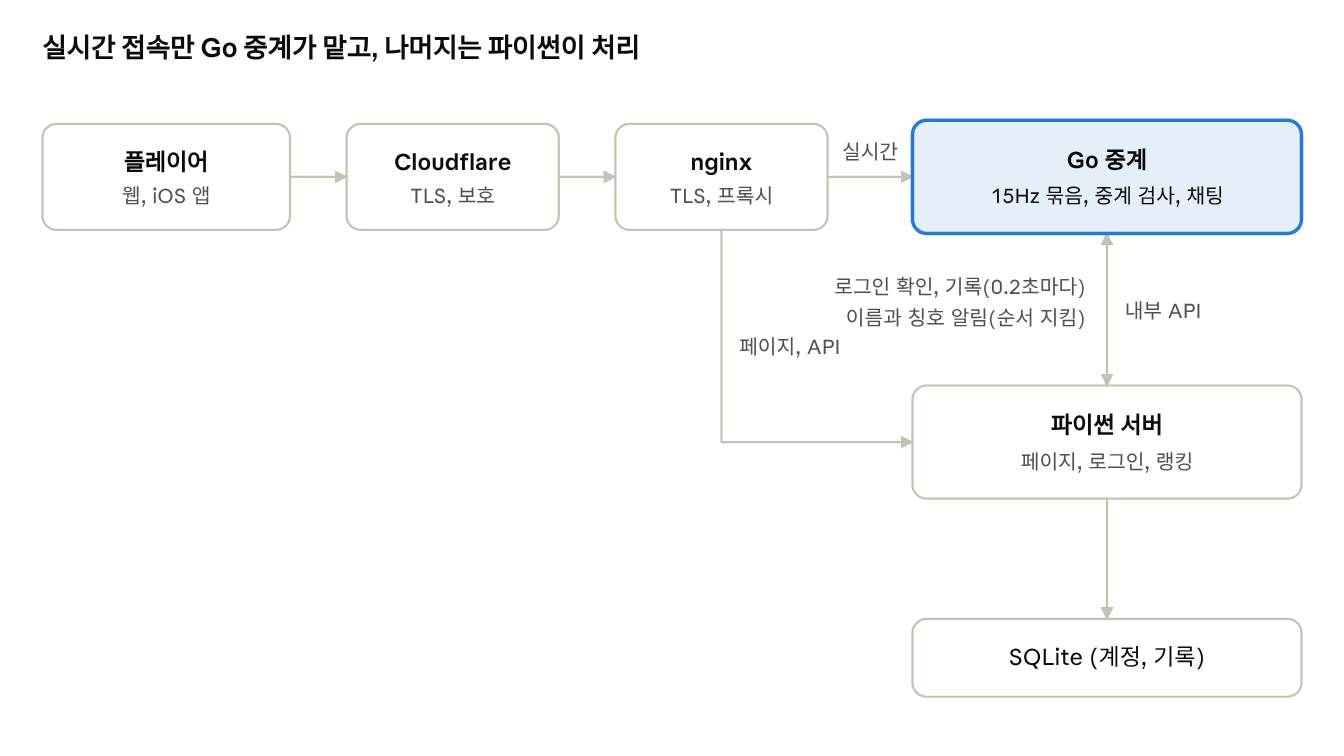
\includegraphics[width=\linewidth]{architecture.png}
  \caption{플레이어 접속 경로. nginx는 실시간 트래픽을 Go 중계로, 페이지와 API 요청을 파이썬으로 보낸다. SQLite는 파이썬이 처리한다. 운영 서버 부하 시험 경로는 \ref{sec:limits}절에 기술한다.}
  \label{fig:architecture}
\end{figure}
\FloatBarrier

\section{측정 방법}
측정은 가짜 플레이어(bot)를 생성해 서버에 접속시키는 하네스로 수행했다. 하네스는 파이썬으로 먼저 작성했고(\code{server/bench\_net.py}), 운영 서버 측정 시 부하 생성 능력을 높이기 위해 Go로 재작성했다. 가짜 플레이어는 게임 엔진과 동일한 순서로 행동한다. 로비에서 스키장을 선택해 알리고, 슬로프 채널 방(40명)에 입장한 뒤 초당 15회 위치를 전송한다. 위치는 실제 시계를 따라 변화하고 속도 값도 해당 움직임에 맞춰 서버의 비정상 이동 검사에 걸러지지 않게 했다. 전송 시점은 참여자마다 위상을 달리한 고정 간격(시작 시각 \(+ k/15\)초)이다.

\begin{itemize}
  \item \textbf{지연.} 방마다 1명의 탐침(probe)이 다른 참여자가 보낸 위치를 수신하기까지 걸린 시간이다. 송수신이 같은 프로세스 내에서 일어나 시계 정합이 불필요하며, 15\,Hz 프레임 대기 시간(평균 33\,ms)이 포함된다.
  \item \textbf{갱신 횟수.} 탐침이 1초에 수신한 방 갱신 수다. 정상값은 15다.
  \item \textbf{송수신량.} 접속별 송수신 바이트를 센다. WebSocket 프레임 헤더를 포함하고 TCP/IP 헤더를 제외한다.
  \item \textbf{서버 CPU.} \code{/proc}에서 Go 중계, 파이썬, nginx를 분리 측정했다. 운영 서버에서는 시스템 전체도 측정했다. 코어 하나를 100\%로 정규화했다.
  \item \textbf{안정성.} 끊긴 접속 수와 방 입장 거부 수다.
\end{itemize}

표~\ref{tab:environments}에 측정 환경 세 곳을 정리했다. 각 단계는 8초 예열 후 30초간 측정했다. 대부분 단계는 1회 측정했고, 운영 서버의 600명과 800명 단계는 2회 측정해 범위로 표기했다(\ref{sec:limits}절). 운영 서버 측정 시 하네스 두 대만 접속 가능한 임시 경로를 개방했다가 종료 후 폐쇄했고, 가짜 플레이어는 실제 플레이어가 사용하지 않는 채널에만 입장시켰다.

\begin{table}[!htbp]
  \caption{측정 환경. 날짜는 2026년 기준이다.}
  \label{tab:environments}
  \small
  \begin{tabularx}{\linewidth}{@{}P{0.22\linewidth}P{0.18\linewidth}L P{0.21\linewidth}@{}}
    \toprule
    \textbf{환경} & \textbf{CPU} & \textbf{서버와 하네스 배치} & \textbf{용도} \\
    \midrule
    운영 서버 (11월 14일) & Ampere 2코어 & 다른 서버 2대(STAGE, 봇 서버)에서 실제 네트워크와 nginx를 경유 & 운영 서버 한계 측정 \\
    Ubuntu i5-11600K (11월 11일) & 서버를 2코어에 바인딩 & 같은 컴퓨터, 다른 코어 & 파이썬 서버 한계 측정 \\
    STAGE (11월 11일) & Ampere 1코어 & 서버와 하네스가 같은 코어 공유 & 두 구현 비교 \\
    \bottomrule
  \end{tabularx}
\end{table}
\FloatBarrier

\section{최적화 과정}
병목은 대역폭, 파일 핸들, 파이썬 GIL, nginx와 커널 네트워크 처리 순으로 이동했다.

\subsection{변경 필드만 전송하는 델타 인코딩}
기존 구현은 매 갱신마다 위치 전체를 전송했다. 최초 1회만 전체 상태(\code{u})를 보내고 이후 변경된 필드만(\code{v}) 보내도록 수정했다. 표~\ref{tab:delta}는 STAGE 1코어에서 동일 조건으로 비교한 결과다.

\begin{table}[!htbp]
  \caption{STAGE에서 델타 인코딩 적용 전후의 트래픽.}
  \label{tab:delta}
  \small
  \begin{tabular*}{\linewidth}{@{\extracolsep{\fill}}rrr@{}}
    \toprule
    \textbf{동시 접속} & \textbf{1인당 수신량 (KB/s)} & \textbf{서버 송신 (MB/s)} \\
    \midrule
    \DeltaRows
    \bottomrule
  \end{tabular*}
\end{table}

수신량과 서버 송신이 56--60\% 감소했다. 서버가 계속 프레임을 조립하고 검증해야 하므로 CPU 사용량은 거의 변하지 않았다. 이 결과는 관심 영역 관리~\cite{boulanger_2006_10}와 증분 상태 전송~\cite{orsten_2011_4} 연구에서 보고한 트래픽 절감 효과와 부합한다.

\subsection{파일 핸들 누수 수정}
측정 중 동시 접속 약 330명에서 \code{/ws}가 HTTP 500 오류를 발생했다. 접속 처리 함수가 접속 종료 시까지 반환하지 않는 구조에서 SQLite 연결이 닫히지 않고 남은 것이 원인이었다. 접속 하나가 파일 핸들 세 개를 점유하여 기본 한도 1,024개에 도달했다. 데이터베이스 연결을 즉시 닫도록 수정한 뒤에는 접속당 소켓 하나만 사용하며, 100명 기준 점유 파일 핸들이 305개에서 104개로 감소했다. 수정 후 330명 부근의 접속 오류는 재현되지 않았다.

\subsection{접속 한도 상향}
서버 동시 접속 한도를 400명에서 2,000명으로, nginx \code{worker\_connections}를 8,192로, systemd 서비스의 \code{LimitNOFILE}을 65,536으로 상향했다. 이후 CPU가 병목이 되었다.

\subsection{GIL 한계와 Go 재구현}
Ubuntu 컴퓨터에서 파이썬 서버를 2코어에 바인딩하여 재측정한 결과 CPU가 125--133\%에서 더 상승하지 않았다(표~\ref{tab:ubuntu}). 파이썬은 GIL 때문에 파이썬 코드를 동시에 한 스레드만 실행하므로, 두 번째 코어에서 얻는 이득은 약 25\%에 그쳤다.

\begin{table}[!htbp]
  \caption{Ubuntu에서 2코어에 바인딩한 파이썬 서버.}
  \label{tab:ubuntu}
  \small
  \begin{tabular*}{\linewidth}{@{\extracolsep{\fill}}rrrr@{}}
    \toprule
    \textbf{동시 접속} & \textbf{CPU (최대 200\%)} & \textbf{초당 갱신} & \textbf{p50 / p99 (ms)} \\
    \midrule
    \UbuntuRows
    \bottomrule
  \end{tabular*}
\end{table}

이 컴퓨터와 운영 서버의 코어 속도 차이(약 1.75배)를 반영하면 파이썬 기준 운영 서버는 약 450명까지 원활하고 570명 부근에서 한계에 도달할 것으로 추정되었다. 이에 따라 실시간 중계(방 관리, 위치 프레임 조립, 중계 검사, 채팅, 파티)만 Go로 이전하고 페이지, 로그인, 랭킹, 데이터베이스는 파이썬에 유지했다. 표~\ref{tab:stage}는 동일 STAGE 1코어에서 두 구현을 비교한 결과다.

\begin{table}[!htbp]
  \caption{STAGE 1코어에서 파이썬과 Go 비교. 각 구현의 초당 갱신 횟수와 p99 지연(ms)을 표시했다.}
  \label{tab:stage}
  \small
  \begin{tabular*}{\linewidth}{@{\extracolsep{\fill}}rrrr@{}}
    \toprule
    \textbf{동시 접속} & \textbf{파이썬} & \textbf{Go} & \textbf{CPU (파이썬에서 Go로)} \\
    \midrule
    \StageRows
    \bottomrule
  \end{tabular*}
\end{table}

1인당 CPU는 파이썬 0.185\%, Go 0.083\%로 약 2.2배 차이가 났다. 800명에서 Go의 지연 상승은 STAGE의 단일 코어를 하네스와 공유했기 때문이다. Go 중계는 2026년 11월 12일부터 운영 서버에서 가동 중이다.
\FloatBarrier

\section{운영 서버 실측 결과}
\label{sec:results}
본 보고서는 초당 갱신 15회가 유지되고 위치 전달 지연 p99가 150\,ms 이내인 경우를 원활로 정의한다. 150\,ms 상한은 기준 게임에서 종단 간 지연 150\,ms 미만이 거의 인지되지 않았다는 실험~\cite{nister_compact_game_data}과 \emph{Quake 3} 플레이어가 150--180\,ms보다 낮은 핑의 서버를 선호했다는 관측~\cite{armitage_2003_9}에 근거한다. 허용 지연은 장르와 상호작용 유형에 따라 달라지므로~\cite{raaen_2014_3}, 여기서는 하네스로 잰 위치 전달 지연의 판정 기준으로 삼았다.

11월 14일 운영 서버는 700명에서 기준을 충족했다(p99 114\,ms, 초당 15.0회 갱신). 800명에서 CPU 합계가 189--197\%(최대 200\%)에 도달했고 p99는 163--275\,ms로 상승했다. 1,000명부터 p99가 초 단위로 급등했다. 표~\ref{tab:production}에 단계별 수치를, 그림~\ref{fig:capacity}에 지연과 CPU 추이를 제시한다.

\begin{table}[!htbp]
  \caption{2026년 11월 14일 운영 서버 부하 시험. 600명과 800명은 두 차례 측정값의 범위를 표시했다.}
  \label{tab:production}
  \small
  \begin{tabular*}{\linewidth}{@{\extracolsep{\fill}}rrrrrr@{}}
    \toprule
    \textbf{동시 접속} & \textbf{초당 갱신} & \textbf{p50 / p99 (ms)} &
    \shortstack[r]{\textbf{CPU 합계}\\(최대 200\%)} & \textbf{Go 중계} & \textbf{nginx} \\
    \midrule
    \ProductionRows
    \bottomrule
  \end{tabular*}
\end{table}

모든 단계에서 접속 끊김과 방 입장 거부는 발생하지 않았다. 한계를 넘으면 서버는 연결을 유지하면서 전송이 늦어진다. 800명에서 1인당 수신량이 13--21\% 감소했고 1,000명 이상에서는 절반 가까이 감소했다.

1인당 CPU 비용은 Go 중계 약 0.14\%, nginx 약 0.10\%였다. nginx의 1인당 CPU 사용량은 중계 프로그램의 약 70\%였다.\footnote{작성 당시 한글 PDF의 ‘약 70\% 더 많은’을 정정했다. 1인당 CPU 비용과 700명 단계의 실측값(nginx 73\%, Go 101\%)이 모두 약 70\%의 비율을 뒷받침한다.} 나머지 CPU 사용량은 주로 커널 네트워크 처리 때문이었다. 파이썬 서버는 0--1\%로 사실상 유휴했는데, 가짜 플레이어가 게스트여서 로그인 검증과 기록 전송이 없었기 때문이다. 하네스 두 대의 CPU는 1,200명에서도 66--72\%에 그쳐, 한계는 서버 측에 있었다.

Go 적용 후 실측한 원활 한계는 파이썬 추정치 450명의 약 1.5배였다. 중계 자체는 STAGE에서 1인당 CPU 효율이 약 2.2배 개선되었다. nginx와 커널 비용이 그대로 남아 전체 수용 인원의 개선 폭은 그보다 작았다.

\ReportFigure{prod-capacity.png}
  {위치 전달 지연(위, 로그 눈금)과 CPU 사용량(아래). 점선은 원활 기준을 충족한 최대 시험 부하를 나타낸다. 600명과 800명의 CPU 막대는 두 차례 측정의 평균이다.}
  {fig:capacity}

\section{논의}
\textbf{병목의 이동과 잔존 비용.}
최적화 과정에서 병목은 대역폭, 파일 핸들, GIL, nginx와 커널 순으로 이동했다. 각 단계의 해법이 다음 병목을 드러냈다. 중계가 가벼워진 뒤에는 리버스 프록시와 커널이 남은 CPU 비용의 상당 부분을 차지했다. 구현 언어를 바꿨을 때 시스템 전체의 개선 폭은 해당 구성 요소의 개선 폭보다 작을 수 있다.

\textbf{측정 방법론의 함정.}
시험 구성의 세 가지 요소가 결과에 영향을 주었다. 첫째, 초기 하네스가 ‘전송 후 1/15초 휴지’를 반복하자 봇이 서버 틱 직후에 몰려 전송했고, 지연이 61\,ms로 부풀려졌다. 참여자마다 위상이 다른 고정 간격 전송으로 해결했다. 실제 플레이어는 기기가 서로 달라 이렇게 동기화되지 않는다. 둘째, 동일 1코어에서는 하네스가 Go 중계보다 CPU를 더 사용했다. 파이썬 하네스는 1코어에서 약 300명이 한계였고, 운영 서버 측정용 Go 하네스는 약 650명까지 생성할 수 있었다. 셋째, 동일 머신 내 측정값은 네트워크를 거친 운영 서버보다 작게 나왔다. STAGE에서 1인당 0.083\%였던 Go 중계 CPU 비용은 운영 서버에서 0.14\%였다. 동일 머신 수치는 구현 비교에 사용했고, 운영 서버의 수용 인원은 네트워크를 거친 시험에서 판단했다. 저인원 구간에서는 고정 비용 때문에 1인당 비용이 크게 보이므로 1인당 비용은 200명 이상 결과로 산출했다. 이러한 보정 원칙은 봇 기반 측정으로 실측을 근사하기 위한 문헌의 조건과 맞닿아 있다~\cite{boulanger_2006_10}.

\textbf{문헌과의 대비.}
관심 영역 관리 문헌은 가시성과 장애물을 고려한 필터링으로 메시지량을 크게 줄인다~\cite{boulanger_2006_10}. 본 시스템은 방(채널) 단위의 단순한 공간 분할로 충분했다. 스키장에서는 시야 차폐가 게임플레이에 미치는 영향이 작고, 40명 규모 방에서는 전원 방송의 비용이 필터링의 계산 비용보다 낮기 때문으로 해석된다. \ref{sec:results}절에서 갱신 빈도가 초당 15.0회에서 12.7회로 떨어지고 수신량도 줄어든 것은, 포화 시 전송 지연이 사실상의 역압(backpressure)으로 작동했음을 시사한다. 갱신을 적응적으로 걸러 대역폭 할당량을 지키는 접근~\cite{gascon_samson_2015_6}과는 메커니즘이 다르다.
\section{한계}
\label{sec:limits}
\begin{itemize}
  \item \textbf{TLS 미포함.} 운영 서버 측정은 nginx까지 평문(HTTP)으로 진행했다. 실제 플레이어는 Cloudflare와 TLS를 거치므로 해당 경로에서는 수용 인원이 낮아질 수 있다.
  \item \textbf{실제보다 무거운 부하 프로파일.} 가짜 플레이어는 휴식 없이 활동했고 방이 항상 40명으로 가득 찼다. 실제로는 메뉴나 리프트권 화면에서 위치를 전송하지 않고 방이 덜 찬다. 이 조건에서는 실제보다 보수적인 결과다.
  \item \textbf{반복 측정 부족.} 대부분 단계가 1회 측정이다. 800명의 두 p99(163\,ms와 275\,ms) 차이가 컸던 것처럼 한계 근처에서는 작은 변동에도 결과가 크게 흔들린다.
  \item \textbf{검증 범위.} 충돌 판정은 서버 단위 테스트로 확인했다. 위치 전달, 채팅, 파티는 실제 게임 화면으로 확인했다.
\end{itemize}

\section{결론 및 향후 계획}
보고서 작성 시점의 실제 동시 접속은 수 명 수준이므로 시험한 상한까지 여유가 충분하다. 접속이 증가하면 다음 우선순위로 대응한다.

\begin{enumerate}
  \item \textbf{nginx 우회.} Cloudflare Origin Rules로 \code{/ws}만 다른 포트의 Go 중계로 직접 전달하고 TLS는 Go가 처리한다. 플레이어 접속 주소와 iOS 앱은 유지할 수 있다. 700명 단계에서 nginx가 사용하던 전체 CPU의 약 40\%를 확보해 900--1,000명을 기대한다. IP당 접속 속도 제한, 느린 연결 차단, \code{CF-Connecting-IP} 기반 실제 IP 식별, 인증서 관리를 Go 측으로 이전해야 한다. 필요한 Origin Rules를 무료 요금제에서 사용할 수 있는지는 미확인이다.
  \item \textbf{전송량 감소.} 숫자 자릿수를 줄이면 수정 범위를 작게 유지하면서 바이트를 20--30\% 줄일 수 있다. 갱신 빈도를 15\,Hz에서 10\,Hz로 낮추면 전송 횟수와 바이트가 1/3 감소하며, 화면 매끄러움에 미치는 영향을 먼저 확인해야 한다. 거리별로 전송 빈도를 달리하면 바이트를 50--70\% 줄일 수 있으나 수신자별 프레임을 생성하므로 CPU 효과는 실측이 필요하다. 기존 형식을 사용하는 배포 완료 iOS 앱과 봇 서버와의 하위 호환을 유지해야 한다.
  \item \textbf{코어 증설.} 마지막 수단으로 유료로 운영 서버 코어를 확장한다.
\end{enumerate}

표~\ref{tab:alternatives}에는 검토한 대안과 채택하지 않은 이유를 정리했다.

\begin{table}[!htbp]
  \caption{검토한 대안과 기각 사유.}
  \label{tab:alternatives}
  \small
  \begin{tabularx}{\linewidth}{@{}P{0.33\linewidth}L@{}}
    \toprule
    \textbf{대안} & \textbf{기각 사유} \\
    \midrule
    서버 전체 Go 이전 & 병목은 실시간 중계에 있었고 페이지와 API 부하는 작았다. \\
    중계를 STAGE(1코어)로 이전 & 원활 한계가 450--550명으로 감소할 것으로 추정되며 시험 서버가 소실된다. \\
    서버 3대에 중계 분산 & 로비, 파티, 채팅의 상태 일관성 유지 비용이 이득보다 크다. \\
    WebSocket 압축 (\code{permessage-deflate}) & 바이트는 감소하나 CPU를 추가 소모해 현재 병목을 악화시킨다. \\
    \bottomrule
  \end{tabularx}
\end{table}

남은 측정 과제는 TLS가 포함된 실제 경로에서의 한계 인원 확인과 nginx 우회 적용 후 재측정이다.
본 보고서는 \href{https://creativecommons.org/licenses/by/4.0/}{CC BY 4.0} 라이선스로 공개한다.
\href{https://github.com/somany-flower4u/multiplayer-perf-report}{프로젝트 저장소}에서 두 언어의 보고서와 그림 원본을 확인할 수 있다.
\FloatBarrier

\bibliographystyle{IEEEtran}
\bibliography{references}
\end{document}
